\section{International Reference Ionosphere (IRI)}

This model has been developed by an international collaboration sponsored by the Committee on Space Research (COSPAR) and the international Union of Radio Science (URSE). The development started in the late sixties in order to create a standardized model of the ionosphere by compiling empirical data from the available sources at the time. this model has been updated several times  in order to keep it up to date with current measurements.
The data of IRI comes ionosondes, incoherent scatter radars, satellites and sounding rockets.
\newline
\newline
A comparison was made between the data from the IRI model and the data obtained with EISCAT's incoherent scatter radar in Svalbard, Norway. This comparison takes data at around 21:01 hours on the 30th of October of 2003, as part of the Halloween solar storms.

\begin{figure}[H]
	\centering
	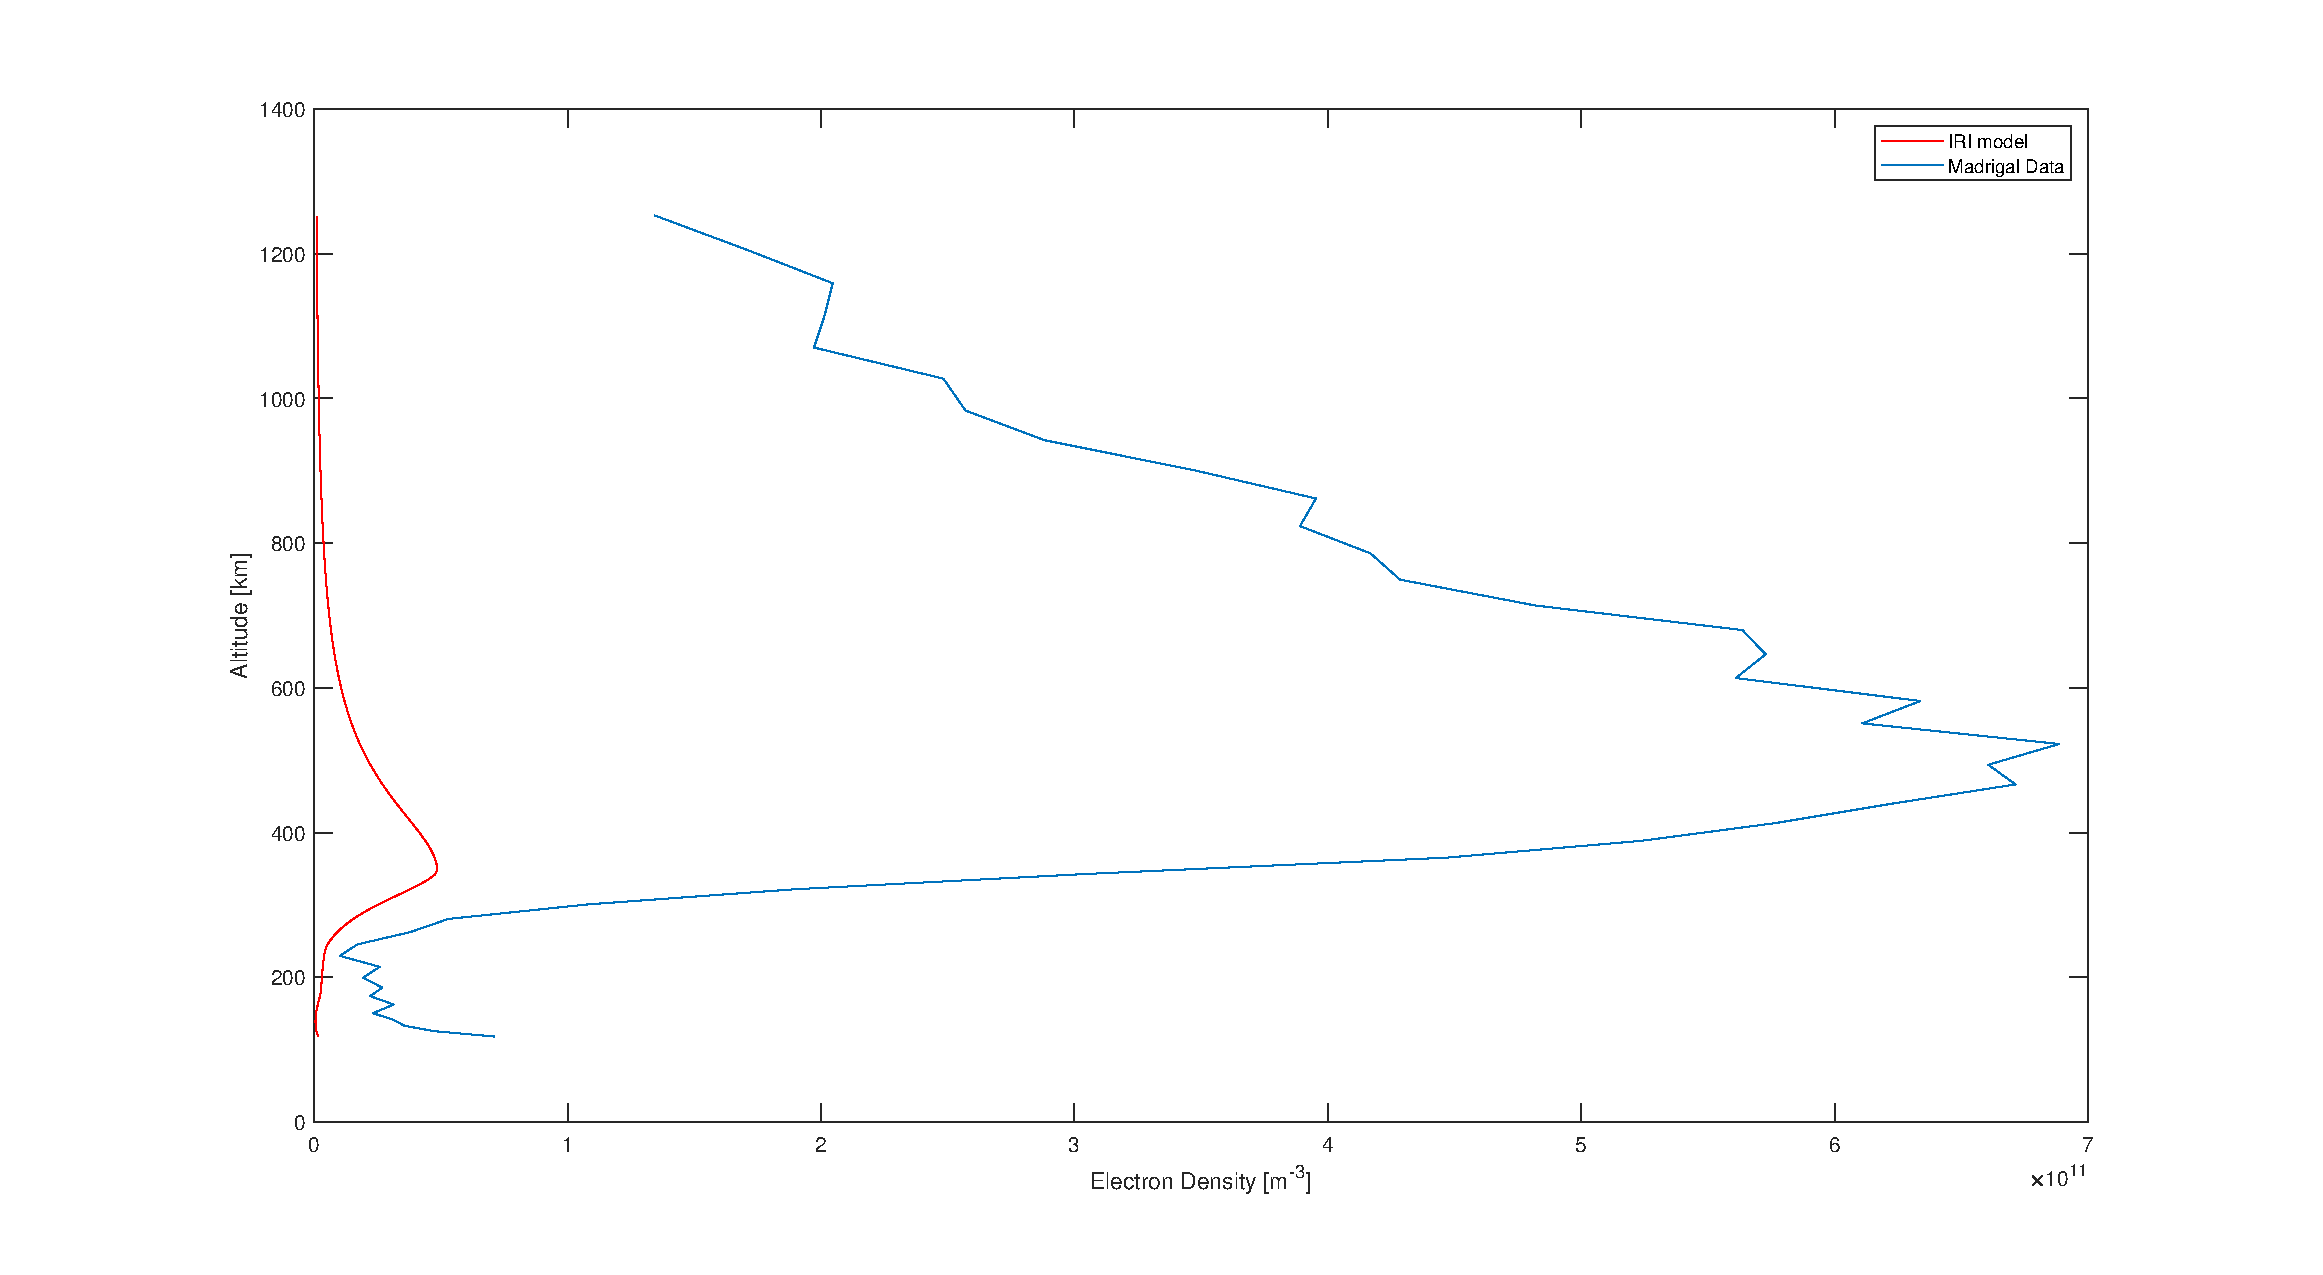
\includegraphics[height=14cm, width=\textwidth]{figures/IRIandMadrigalNe.eps}
	\caption{Comparison of the IRI model data (red) and the one obtained from EISCAT through the Madrigal system (blue).}
	\label{fig::IRIvsMa}
\end{figure}

While both sources more or less agree where the maximum of electron density occurs. There is a big discrepancy in the values shown, of about one order of magnitude.This can be attributed to the fact that the IRI model uses a monthly average to display the electron density of a particular time and date.